% !TeX program = xelatex
% !TeX encoding = UTF-8
\documentclass{JXUSTmodeling}

\usepackage{booktabs}

\biaoti{机器人避障问题讨论}
\keyword{Floyd算法;无向图理论;非线性约束;道路规划}
\begin{document}
\begin{abstract}
本文根据Floyd算法和无向图理论对机器人避障问题推导出相应的避障模型,结合实际情况,进一步利用matlab对避障模型进行求解,针对不同的障碍物和目标点的情况,建立了通用的目标优化模型,得出在有障碍物的情况下,机器人到达目标点所用的最短路径和最短时间。\par
对于问题一,先将平面场景图中的障碍物的顶点与目标顶点抽象成无向图的顶点,令顶点间可直通的路径的长度作为边的权值,进而形成带权无向图,结合Floyd算法和无向图理论等的相关概念,通过matlab计算出路由矩阵和距离矩阵,由路由矩阵得出~$O\to A,O\to B,O\to C$~和~$O\to A\to B\to C\to O$~的最短路径,进而根据距离矩阵和机器人转弯的弧长得出实际最短路径长度。\par
对于问题二,首先判断机器人到达A点的运动情况以及转弯情况,结合牛顿运动公式,逐个分析运动状态,并写出运动模型。通过运动模型,清楚地得出机器人运动的规律,根据机器人应该距离障碍物至少10个单位作为约束条件,把机器人到达A点的总时间作为目标函数,带入matlab计算得出最小时间以及转弯的位置,最终得出所用最短时间约为~$t=94s$。\par
对于上述模型的建立,通过对数据的分析,与实际情况大致相符,说明模型的可靠性较高。
\end{abstract}
\section{问题的提出}\label{sec:1}

在~$800\times 800$~的平面场景图中,远点处有一个只能平面活动的机器人,在保障机器人正常行走并绕过障碍物,要求到达目标点与障碍物的距离至少超过10个单位,且规定机器人的行走路径由直线段和圆弧构成,圆弧是机器人的转弯路径。机器人不能折现转弯,转弯路径由与直线相切的一段圆弧组成,也可由多段相切圆弧组成,但每个圆弧半径最小10个单位。机器人行走最大速度为5个单位/秒。用数学建模确定机器人到达目的地的最短路径和最短时间,并解决一下问题:
\begin{enumerate}
\item 分别求出~$O\to A,O\to B,O\to C$~和~$O\to A\to B\to C\to O$~的最短路径。
\item ~$O\to A$~的最短时间。
\end{enumerate}

\section{问题的分析}\label{sec:2}
\subsection{问题的整体分析}\label{sub:2.1}
伴随着科技的进步和生活质量的提高,机器人也逐渐走入我们的生活,特别是一些高档的酒店用机器人代替人的服务,这就对机器人的程序要求越来越高,本题主要模拟机器人在有障碍物的情况下,如何进行适当的选择路径以保证路径最短或时间最短。
\subsection{问题一的分析}\label{sub:2.2}
对于问题一,考虑到两点之间的距离,直线的长度比弧线短,因此机器人走弧线往往是调整方向,又因为机器人要避障,在避障处需要改变轨迹,机器人只能走直线和圆弧。综合考虑,机器人在顶点处转弯处是求取最短路径的最佳选择,且转弯圆半径为最小10个单位。找到每个障碍物的顶点,根据分析,两个顶点间的距离是可以等效为机器人的行走路径。通过Floyd算法得到所有点的最短路径。而所求点到障碍顶点的距离并不等效为机器人但通过勾股定理易得。 此时将所求的点坐标写入程序中,便可求得最短距离。
\subsection{问题二的分析}\label{sub:2.3}
对于问题二,由于原点到A点之间只有一个障碍物,机器人只能从障碍物5的左侧或下侧绕过,且必须经过一次转弯到达A点,根据机器人与障碍物之间保持一定举例,可以得到约束条件,运用MATLAB便可求出到达A点的最短时间路径。
\newpage
\section{问题的假设}\label{sub:3}
\begin{enumerate}
  \item 假设机器人从静止状态到运动状态产生的加速度为~$1 \ m/s^2$。
  \item 题目中所给数据真实有效。
\end{enumerate}
\section{模型的符号说明}\label{sub:4}

% 三线表写法
\begin{table}[htbp]
  \centering
  %\caption{表注}\label{tab:example}
    \begin{tabularx}{\textwidth}{YY}
    \toprule
    符号 & 物理意义\\
    \midrule
    $a$ & 加速度\\
    $s$ & 路程\\
    $v$ & 速度\\
    $t$ & 时间\\
    $\theta$ & 转弯时走过圆弧的圆心角\\
    $r$ & 转弯时圆弧的半径\\
    \bottomrule
  \end{tabularx}
\end{table}

\section{模型的建立与求解}\label{sec:5}
\subsection{相关概念}\label{sec:5.1}
\subsubsection{Floyd算法}\label{sec:5.1.1}
设~$D_{i,j,k}$~为从~$i$~到~$j$~的只以~$(1\dots k)$~集合中的节点为中心节点的最短路径的长度。\\
若最短路径经过点~$k$~,则
\begin{equation}
  D_{i,j,k} = D_{i,k,k-1}+D_{k,j,k-1};
\end{equation}
若最短路径不经过点~$k$~,则~$D_{i,j,k}=D_{i,j,k-1}$~,因此
\begin{equation}
  D_{i,j,k}=min(D_{i,j,k-1},D_{i,j,k-1}+D_{i,j,k-1}).
\end{equation}
\subsubsection{无向图}\label{sec:5.1.2}
一张图~$G$~是一个二元组~$(V,E)$~,其中~$V$~称为顶点集,~$E$~称为边集。它们亦可写成~$V(G)$~和~$E(G)$。
~$E$~的元素是一个二元组数对,用~$(x,y)$~表示,其中~$x,y\in V$。
\subsubsection{牛顿运动公式}\label{sec:5.1.3}
机器人在运动过程中,经历加速和减速运动,速度与加速度的关系为:
\begin{equation}
  v=v_0+at,
\end{equation}

路程与加速度的关系为:
\begin{equation}
  s= v_0 t+ \frac{1}{2} at^2.  
\end{equation}

\subsection{问题一中模型的建立与解决}\label{sec:5.2}
\subsubsection{网的建立}\label{sec:5.2.1}
题目所给的~$800\times 800$~的平面场景图,其障碍物的数学描述由题目所给的表所示。因机器人在避障的过
程中主要走向为障碍物的顶点,即我们将障碍物的顶点进行标号,顶点之间存在边,用图~$G$~表示,~$V(G)$~表示
图~$G$~的顶点,~$V(G)=\{1,2,3,\cdots,34,35,36,37,38\}$~,其中~$\{1,\cdots,34\}$~为图中障碍物的顶点标号,~$\{35,36,37,38\}$~分别
表示~$O,A,B,C$~四个目标顶点,~$E(G)$~表示为图~$G$~的边,且满足以下公式:
\begin{equation}
  E(G) = 
  \begin{cases}
    l_i & \mbox{,当~$v_i$~与~$v_j$~间有边时} \\
    \infty & \mbox{,当~$v_i$~与~$v_j$~间无边时}
  \end{cases}
\end{equation}
$l_i$~为~$<v_i,v_j>$~边的权值,其值为~$v_i$~顶点与~$v_j$~顶点间的距离。\par
即将平面场景图简化为带权无向图~$G$~,并以领接矩阵~$B$~表示图~$G$~。

% % 图插入
% \begin{figure}[htbp]
%   \centering
%   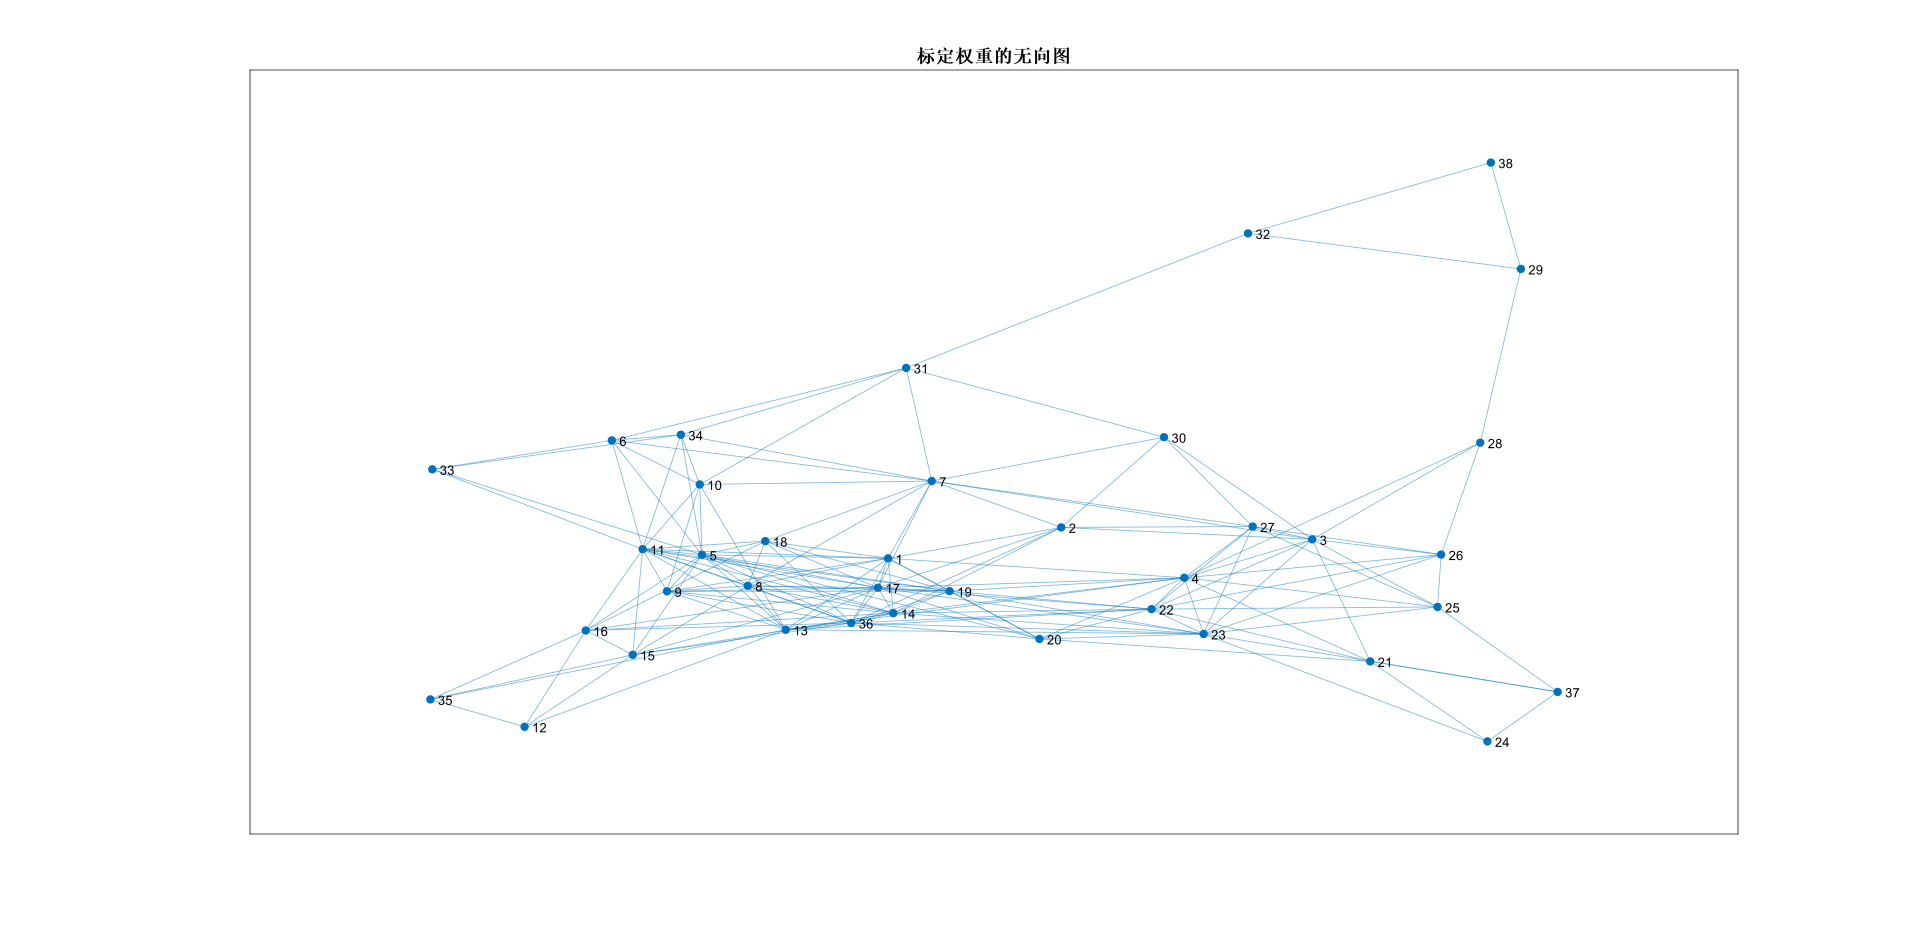
\includegraphics[width=0.4\textwidth]{figures/graph.svg}
%   \caption{图注}\label{fig:example}
% \end{figure}

\subsubsection{路径距离模型}\label{sec:5.2.2}
\begin{enumerate}
  \item 情况一:障碍顶点间机器人行走的距离
  \begin{equation}
    L_1 = l_1 + l_2 + l_3 = l'_1 + \frac{1}{2}r\theta + l'_3,
  \end{equation}
  \item 情况二:目标顶点与障碍顶点间机器人行走的距离
  \begin{equation}
    L_2 = \sqrt{l'^2_1 + r^2} + \frac{1}{2}r\theta + l'_3.
  \end{equation}
\end{enumerate}
\subsubsection{对于障碍物2的路径模型}\label{sec:5.2.3}
得到无向图后,根据障碍顶点坐标和障碍形状分析,通过matlab求解,找到任意两点间的所有直通通路。之后再对编号为2的图形进行处理,找到能够直线到达圆上的障碍顶点,分别为~$\{2,3,7,27,30,31\}$~,假定这些点尽管没有直通通路,但可以借助圆形轨道到达。
\subsubsection{Floyd算法求解模型}\label{sec:5.2.4}
令
\begin{equation}
  D^1 = (d_{ij}^{(1)})_{n\times n},
  d_{ij}^{(1)}=min\{d_{ij}^{(0)},d_{i1}^{(0)}+d_{1j}^{(0)}\}.
\end{equation}
元素~$d_{ij}^{(1)}$~是从~$v_i$~到~$v_j$~中间点只允许为~$v_1$~路径中的最短路长度。

\begin{equation}
  D^2 = (d_{ij}^{(2)})_{n\times n},\\
  d_{ij}^{(2)}=min\{d_{ij}^{(1)},d_{i1}^{(1)}+d_{1j}^{(1)}\}.
\end{equation}
元素~$d_{ij}^{(2)}$~是从~$v_i$~到~$v_j$~中间点只允许为~$v_1,v_2$~路径中的最短路长度。\par
以此类推
$$
\vdots
$$
\begin{equation}
  D^k = (d_{ij}^{(k)})_{n\times n},\\
  d_{ij}^{(k)}=min\{d_{ij}^{(k-1)},d_{i1}^{(k-1)}+d_{1j}^{(k-1)}\}.
\end{equation}
元素~$d_{ij}^{(k)}$~是从~$v_i$~到~$v_j$~中间点只允许为~$v_1,v_2,\cdots,v_k$~路径中的最短路长度。

\subsubsection{模型的结论}\label{sec:5.2.5}
将~$O,A,B,C$~坐标输入,找出与这四个点中能够有直通通路的障碍顶点,通过matlab得出新的距离矩阵和路由矩阵。
$O\to A,O\to B,O\to C$~和~$O\to A\to B\to C\to O$~的最短路径为:\par
$O-A$ : $O-15-A$\par
$O-B$ : $O-16-18-19-20-21-B$\par
$O-C$ : $O-13-11-6-31-32-C$\par
$O-A-B-C-O$ : $O-15-A-20-21-B-23-27-28-29-C-32-31-6-11-13-O$\par


最短路径距离如下表:

\begin{table}[htbp]
  \centering
  \caption{最短路径距离}\label{tab:1}
    \begin{tabularx}{\textwidth}{YY}
    \toprule
    $O-A$ & 474.0348\\
    $O-B$ & 872.3173\\
    $O-C$ & 1116.7\\
    $O-A-B-C-O$ & 2922.2\\
    \bottomrule
  \end{tabularx}
\end{table}

\subsection{问题二中模型的建立与解决}\label{sec:5.3}

\section{模型的检验}\label{sec:6}
机器人在帮助人类完成一些简单的工作时,效率总是第一要素。因此,机器人在正常行走过程中,使用最短路径,耗费最少的时间成为提高效率的决定性。
对于问题一中,运用……方法时,存在……缺陷,导致……误差,因此求解时还可以选取……方法进行分析。
对于问题二中,运用了matlab线性分析,把障碍物坐标作为约束条件,约束条件中存在计算不精准的误差,因此求解时还可以考虑使约束条件更加精确的分析方法。


\section{模型的评价及推广}\label{sec:7}
\subsection{模型的优点}\label{sec:7.1}
\begin{enumerate}
  \item 本文运用了迪特科斯拉算法和无向图理论,清楚地分析了机器人走每一条路时的权,对比权重得直观可靠的最短路径,具有较强的说服力和可靠性。
  \item 本文整体分析了最短时间的可能条件,利用matlab精准地找到了机器人转弯时的圆心坐标以及半径,模型形式简单,便于理解。
  
\end{enumerate}
\subsection{模型的缺点}\label{sec:7.2}
\begin{enumerate}
  \item 在问题一中,在寻找最短路径的Floyd算法中,当机器人经过障碍物的顶点时,并未完全考虑到机器人行走线路与障碍物间的最近距离为10个单位所带来的影响。
  \item 在问题一中,在领接矩阵中,机器人从目标点与障碍顶点之间的转弯弧长长度有一定偏差。
  \item 针对问题二,机器人转弯时旋转自身方向的时间考虑的不够全面,忽略自身旋的时间,对最短时间可能造成一定的误差。
  
\end{enumerate}

\subsection{模型的改进}\label{sec:7.3}
\begin{enumerate}
  \item 在问题一中,提高避障最短路径的数学模型通用性。
  \item 在问题二中,应该采用更加精准的约束条件,从而使求得的对短时间更加精准。
\end{enumerate}

\begin{thebibliography}{99}
  \bibitem{label}参考文献
\end{thebibliography}

\begin{appendixx}
  \section{问题一的 MATLAB 代码}
  \subsection{主文件}
  \begin{matlab}
    clc,clear

% 领接矩阵数据填充
clc,clear
B = inf(38,38);
for i = 1:38
    B(i,i) = 0;
end
a=[300 500 500 300 360 500 540 400 280 410 345 80 230 230 80 60 235 150 220 220 150 240 270 180 370 430 540 670 540 640 720 720 500 500 0 300 100 700]; 
b=[400 400 600 600 240 240 330 330 100 100 210 60 60 210 210  300 300 435 470 530 600 600 680 680 680 680 600 730 730 520 520 600 140 200 0 300 700 640];
for i=[1,5,8,11,14,17,19]
    for j=[1,5,8,11,14,17,19]
    B(i,j)=getLength(a(i),b(i),a(j),b(j)); 
    end
end
for i=[20 21 22 4]
    for j=[20 21 22 4]
    B(i,j)=getLength(a(i),b(i),a(j),b(j)); 
    end
end
for i=[3 23 25 26 27 4]
    for j=[3 23 25 26 27 4]
    B(i,j)=getLength(a(i),b(i),a(j),b(j)); 
    end
end
for i=[7 31 6 34 10]
    for j=[7 31 6 34 10]
    B(i,j)=getLength(a(i),b(i),a(j),b(j)); 
    end
end
for i=[10 9 13]
    for j=[10 9 13]
    B(i,j)=getLength(a(i),b(i),a(j),b(j)); 
    end
end
for i=[17 18 19 1 8 5 7]
    for j=[17 18 19 1 8 5 7]
    B(i,j)=getLength(a(i),b(i),a(j),b(j)); 
    end
end
for i=[1 2 17 8 7 14]
    for j=[1 2 17 8 7 14]
    B(i,j)=getLength(a(i),b(i),a(j),b(j)); 
    end
end
for i=1:34
    B(16,i)=inf;
end
B(16,18)= getLength(a(16),b(16),a(18),b(18));
for i=[12 15 16]
    for j=[12 15 16]
    B(i,j)=getLength(a(i),b(i),a(j),b(j)); 
    end
end
for i=[15 14 16 17 11 5]
    for j=[15 14 16 17 11 5]
    B(i,j)=getLength(a(i),b(i),a(j),b(j)); 
    end
end
for i=[5 9 11 8 1 17 14 13]
    for j=[5 9 11 8 1 17 14 13]
    B(i,j)=getLength(a(i),b(i),a(j),b(j)); 
    end
end
for i=[13 14 22 23 4]
    for j=[13 14 22 23 4]
    B(i,j)=getLength(a(i),b(i),a(j),b(j)); 
    end
end
for i=[4 17 19 20 22 23]
    for j=[4 17 19 20 22 23]
    B(i,j)=getLength(a(i),b(i),a(j),b(j)); 
    end
end

B(20,1)=getLength(a(1),b(1),a(20),b(20));
B(22,3)=getLength(a(3),b(3),a(22),b(22));
B(28,3)=getLength(a(3),b(3),a(28),b(28));

B(1,20)=getLength(a(1),b(1),a(20),b(20));
B(3,22)=getLength(a(3),b(3),a(22),b(22));
B(3,28)=getLength(a(3),b(3),a(28),b(28));

for i=[1 17 19 28]
    B(4,i)=getLength(a(4),b(4),a(i),b(i));
    B(i,4)=getLength(a(4),b(4),a(i),b(i));
end
for i=[6 10 20 33 34]
    B(5,i)=getLength(a(5),b(5),a(i),b(i));
    B(i,5)=getLength(a(5),b(5),a(i),b(i));
end

B(11,6)=getLength(a(6),b(6),a(11),b(11));
B(33,6)=getLength(a(6),b(6),a(33),b(33));
B(17,7)=getLength(a(7),b(7),a(17),b(17));
B(15,8)=getLength(a(8),b(8),a(15),b(15));
B(19,9)=getLength(a(9),b(9),a(19),b(19)); 

B(6,11)=getLength(a(6),b(6),a(11),b(11));
B(6,33)=getLength(a(6),b(6),a(33),b(33));
B(7,17)=getLength(a(7),b(7),a(17),b(17));
B(8,15)=getLength(a(8),b(8),a(15),b(15));
B(9,19)=getLength(a(9),b(9),a(19),b(19)); 

for i=[5 11 13]
    B(10,i)=getLength(a(8),b(8),a(i),b(i)); 
    B(i,10)=getLength(a(8),b(8),a(i),b(i)); 
end
for i=[8 18 33 34]
    B(11,i)=getLength(a(11),b(11),a(i),b(i)); 
    B(i,11)=getLength(a(11),b(11),a(i),b(i)); 
end
B(12,13)=getLength(a(12),b(12),a(13),b(13)); 
B(13,12)=getLength(a(12),b(12),a(13),b(13)); 
B(21,24)=getLength(a(21),b(21),a(24),b(24)); 
B(24,21)=getLength(a(21),b(21),a(24),b(24)); 
for i=[23 25 26 27]
    B(i,22)=getLength(a(22),b(22),a(i),b(i)); 
    B(22,i)=getLength(a(22),b(22),a(i),b(i)); 
end

B(24,23)=getLength(a(23),b(23),a(24),b(24)); 
B(28,26)=getLength(a(26),b(26),a(28),b(28)); 
B(28,27)=getLength(a(28),b(28),a(28),b(28)); 
B(30,27)=getLength(a(27),b(27),a(30),b(30));
B(29,28)=getLength(a(28),b(28),a(29),b(29)); 
B(32,29)=getLength(a(29),b(29),a(32),b(32)); 
B(31,30)=getLength(a(30),b(30),a(31),b(31)); 
B(32,31)=getLength(a(31),b(31),a(32),b(32));
B(34,33)=getLength(a(33),b(33),a(34),b(34)); 
B(3,21)=getLength(a(21),b(21),a(3),b(3)); 
B(8,2)=inf;
B(7,5)=inf;
B(14,7)=inf;
B(19,7)=inf;



B(23,24)=getLength(a(23),b(23),a(24),b(24)); 
B(26,28)=getLength(a(26),b(26),a(28),b(28)); 
B(27,28)=getLength(a(28),b(28),a(28),b(28)); 
B(27,30)=getLength(a(27),b(27),a(30),b(30));
B(28,29)=getLength(a(28),b(28),a(29),b(29)); 
B(29,32)=getLength(a(29),b(29),a(32),b(32)); 
B(30,31)=getLength(a(30),b(30),a(31),b(31)); 
B(31,32)=getLength(a(31),b(31),a(32),b(32));
B(33,34)=getLength(a(33),b(33),a(34),b(34)); 
B(21,3)=getLength(a(21),b(21),a(3),b(3)); 
B(2,8)=inf;
B(5,7)=inf;
B(7,14)=inf;
B(7,19)=inf;


% 添加O,A,B,C点
for i=[12 13 15 16]
    B(35,i) = getLength(a(35),b(35),a(i),b(i));
    B(i,35) = getLength(a(35),b(35),a(i),b(i));
end

for i = [1 2 5 8 9 11 13 14 15 16 17 18 19 20 22 23]
    B(36,i) = getLength(a(36),b(36),a(i),b(i));
    B(i,36) = getLength(a(36),b(36),a(i),b(i));
end

for i = [21 23 24 25]
    B(37,i) = getLength(a(37),b(37),a(i),b(i));
    B(i,37) = getLength(a(37),b(37),a(i),b(i));
end

for i = [29 32]
    B(38,i) = getLength(a(38),b(38),a(i),b(i));
    B(i,38) = getLength(a(38),b(38),a(i),b(i));
end


% 计算经过障碍物2的边
for i = [2 3 7 27 30]
    for j = [2 3 7 27 30] 
        temp = C2Length(a(i),b(i),a(j),b(j));
        if B(i,j) > temp
            B(i,j) = temp;
        end
    end
end


[d,r] = floyd(B)
A = B;
for i = 1:38
    for j = 1:38
        if A(i,j) == inf
            A(i,j) = 0;
        end
    end
end
G=graph(A,'upper');%根据带权邻接矩阵生成无向图
plot(G)
title('标定权重的无向图')


% 计算最短路径的真实距离
% O-A
L1 = getCirLength(a(35),b(35),a(15),b(15),a(36),b(36)) + d(35,36);
% O-B
L2 = getCirLength(a(35),b(35),a(16),b(16),a(18),b(18)) + getCirLength(a(16),b(16),a(18),b(18),a(19),b(19)) + getCirLength(a(18),b(18),a(19),b(19),a(20),b(20)) + getCirLength(a(19),b(19),a(20),b(20),a(21),b(21)) + getCirLength(a(20),b(20),a(21),b(21),a(37),b(37)) + d(35,37);
% O-C
L3 = getCirLength(a(35),b(35),a(13),b(13),a(11),b(11)) + getCirLength(a(13),b(13),a(11),b(11),a(6),b(6)) + getCirLength(a(11),b(11),a(6),b(6),a(31),b(31)) + getCirLength(a(6),b(6),a(31),b(31),a(32),b(32)) + getCirLength(a(31),b(31),a(32),b(32),a(38),b(38)) + d(35,38);
% O-A-B-C-O
L4 = getCirLength(a(35),b(35),a(15),b(15),a(36),b(36)) + getCirLength(a(15),b(15),a(36),b(36),a(20),b(20)) + getCirLength(a(36),b(36),a(20),b(20),a(21),b(21)) + getCirLength(a(20),b(20),a(21),b(21),a(37),b(37)) + getCirLength(a(21),b(21),a(37),b(37),a(23),b(23)) + getCirLength(a(37),b(37),a(23),b(23),a(27),b(27)) + getCirLength(a(23),b(23),a(27),b(27),a(28),b(28)) + getCirLength(a(27),b(27),a(28),b(28),a(29),b(29)) + getCirLength(a(28),b(28),a(29),b(29),a(38),b(38)) + getCirLength(a(29),b(29),a(38),b(38),a(32),b(32)) + getCirLength(a(38),b(38),a(32),b(32),a(31),b(31)) + getCirLength(a(32),b(32),a(31),b(31),a(6),b(6)) + getCirLength(a(31),b(31),a(6),b(6),a(11),b(11)) + getCirLength(a(6),b(6),a(11),b(11),a(13),b(13)) + getCirLength(a(11),b(11),a(13),b(13),a(35),b(35)) + d(35,36) + d(36,37) + d(37,38) + d(38,35);


  \end{matlab}
  \subsection{Foldy算法}
  \begin{matlab}
% d是矩离矩阵
% r是路由矩阵
function [d,r]=floyd(a)
    n=size(a,1);
    % 初始化距离矩阵
    d=a;
    % 初始化路由矩阵
    for i=1:n
        for j=1:n
            r(i,j)=j;
        end 
    end 
    r;

    % Floyd算法开始
    for k=1:n
        for i=1:n
            for j=1:n
                if d(i,k)+d(k,j)<d(i,j)
                    d(i,j)=d(i,k)+d(k,j);
                    r(i,j)=r(i,k);
                end 
            end 
        end
        k;
        d;
        r;
    end
    d
    r
end
  \end{matlab}
  \subsection{距离算法}
  \begin{matlab}
    function [length] = getCirLength(m1,n1,m2,n2,m3,n3)
    g1 = atan((n2-n1)/(m2-m1));
    g2 = atan((n3-n2)/(m3-m2));
    
    g = pi-abs(g1-g2);
    
    length = (1/2) * 10 * g;
    
end
  \end{matlab}
  \begin{matlab}
    function [length] = getLength(m1,n1,m2,n2)
    length = sqrt((m2-m1)^2 + (n1-n2)^2);
end
  \end{matlab}
  \begin{matlab}
    function [length] = C2Length(m1,n1,m2,n2)
    t1 = sqrt(getLength(m1,n1,550,450)^2 - 70^2);
    t2 = sqrt(getLength(m2,n2,550,450)^2 - 70^2);
    t3 = getLength(m1,n1,m2,n2);
    a1 = atan(t1/70);
    a2 = atan(t2/70);
    a3 = acos((getLength(m1,n1,550,450)^2 + getLength(m2,n2,550,450)^2 - t3^2)/(2*getLength(m1,n1,550,450)*getLength(m2,n2,550,450)));
    length = (1/2) * 70 * (2*pi - (a1 + a2 + a3)) + t1 + t2;
end


  \end{matlab}
  \section{问题二的Matlab代码}
  
  \begin{matlab}
    function f = MinTime(x)
    f=5+(((x(1)^2+x(2)^2+x(3)^2))^(1/2)-12.5-5*(5-(5/(1+exp(10-0.1*x(3)))))-((5-(5/(1+exp(10-0.1*x(3)))))^2)/2)/5+2*(5-(5/(1+exp(10-0.1*x(3)))))+(((x(1)-300)^2+(x(2)-300)^2+x(3)^2)^(1/2)-(5/(1+exp(10-0.1*x(3))))*(5-(5/(1+exp(10-0.1*x(3)))))-((5-(5/(1+exp(10-0.1*x(3)))))^2)/2)/5+(atan(x(2)/x(1))-atan((300-x(2))/(300-x(1)))*x(3))/5;
end
  \end{matlab}
  \begin{matlab}
    function Time
x0=[70;220;5];
A = [0 -1 -1;1 0 1;-1 0 1]; 
B = [-210;80;0]; 
Aeq = []; 
beq = [];
lb =[0;150;5];
ub = [80;230;50];
[x,fval]=fmincon(@MinTime, x0 , A , B , Aeq , beq , lb , ub, @con5);

x
fval

  \end{matlab}
  \begin{matlab}
    
function [C,Ceq]=con5(x)
Ceq=[];
C=((x(1)-80)^2+(x(2)-210)^2)^(1/2)-x(3)+10;
  \end{matlab}
\end{appendixx}


\end{document}

